\section{Experiment}
\label{experiment}
\subsection{Setup}
Our experimental data consists of running small programs under 4 different configurations: with contracts and the JIT, with no contracts and the JIT, with contracts and no JIT, and finally with no contracts and no JIT.
We disabled the JIT using the Racket command-line flag \mono{--no-jit} and disabled contracts by editing the \mono{racket/contract} source code\textemdash wherever contracts were applied, we replaced the actual contract with a trivial \mono{any/c} contract.
See \sect{disabling-contracts} for further discussion on how we disabled contracts and the difficulties we faced, but for the moment note that we still incur the cost of making contracts (before they are discarded) and potentially incur a level of indirection for the \mono{any/c} calls even though they automatically accept their argument.

The eight programs we collected data for are taken from Project Euler~\cite{project-euler} and the artifact by Nyugen et~al. on soft contracts~\cite{soft-contracts}.
We wrote the 5 Project Euler (PE) solutions ourselves and added contracts to individual functions exactly how type signatures would guard the functions statically.
These solutions were picked arbitrarily and are not solved in any particular way.\footnote{In fact, a more experienced Racketeer might cringe at our solutions.}
The 3 games we took from the soft contracts repository~\cite{soft-contracts-repo} were implemented as a collection of modules.
Contracts protect module boundaries, but there are no contracts checks within any single module.

We ran each of these 8 benchmark programs on a modern desktop using Racket version 6.1.1.5 and collected the CPU time taken for the run.\footnote{CPU time was obtained by calling Racket's built-in \mono{time} function.}
To address potential outliers, we ran each benchmark 30 times on each configuration of Contracts and JIT.
Note that we started a new Racket VM for each of the 30 runs; our experiment does not measure differences between startup and steady-state performance.

\subsection{Results}

\newpage
\begin{figure}[t]
  \begin{center}
  \vspace*{-2cm}\hspace*{-3.5cm}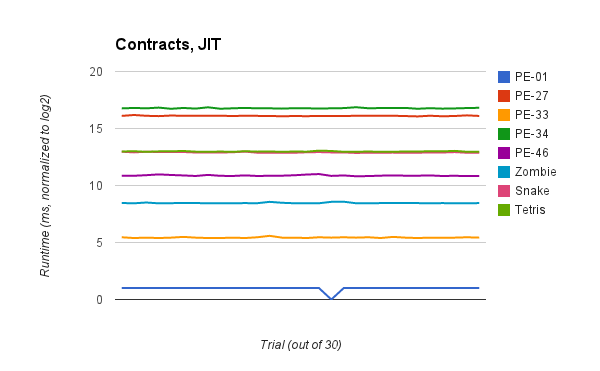
\includegraphics[width=10cm]{data/contracts-jit-runtime.png}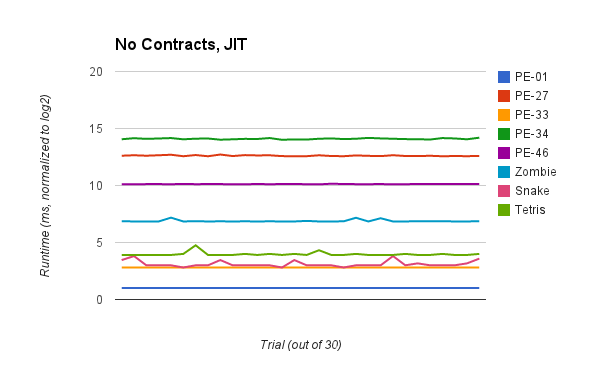
\includegraphics[width=10cm]{data/nocontracts-jit-runtime.png}

  \vspace{1cm}\hspace*{-3.5cm}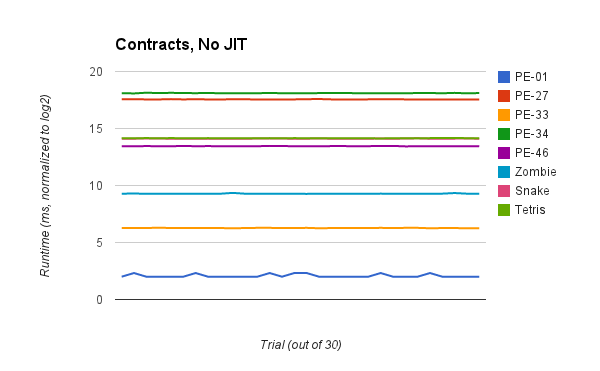
\includegraphics[width=10cm]{data/contracts-nojit-runtime.png}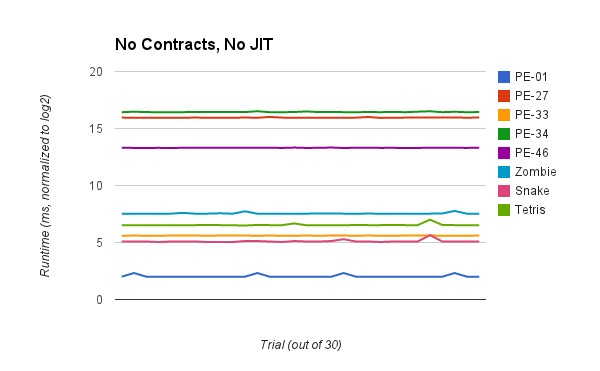
\includegraphics[width=10cm]{data/nocontracts-nojit-runtime.png}
  
  \caption{Experiment runtimes partitioned by Contracts / JIT setting and normalized to $\mathsf{log}_2$. Measurements taken by Racket's \texttt{time} function.}
  \label{trials}
  \end{center}
\end{figure}
\newpage
\begin{figure}[t]
  \begin{center}
  \hspace*{-1.5cm}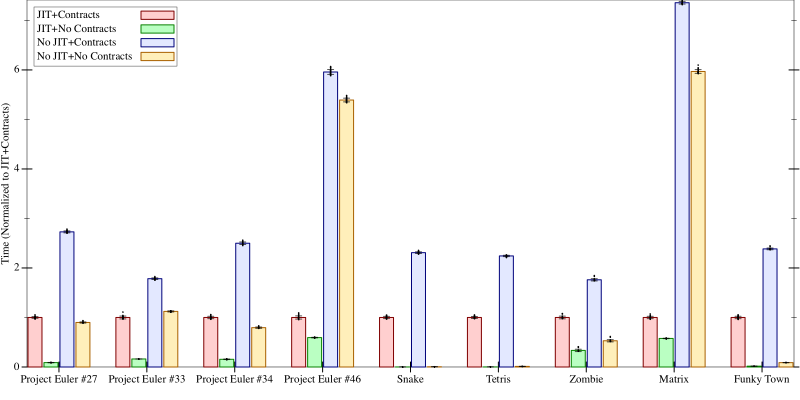
\includegraphics[width=15cm]{data/normalized-runtimes.png}
  \caption{All experiment runtimes, normalized to contracts + JIT runtime.}
  \label{fig:runtimes}
  \end{center}
\end{figure}

\newpage
\begin{figure}[!thb]
  \begin{center}
  \vspace*{-2cm}\hspace*{-1cm}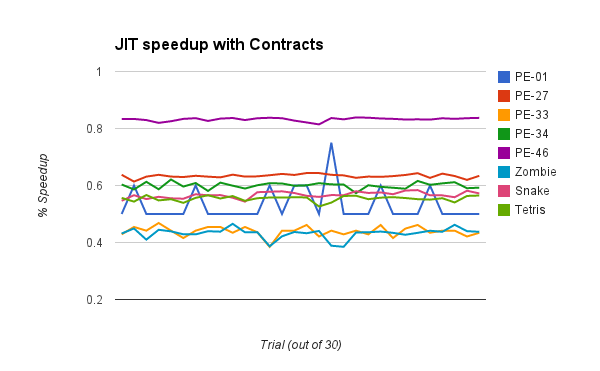
\includegraphics[width=\textwidth]{data/contracts-jit-speedup.png}

  \vspace*{1cm}\hspace*{-1cm}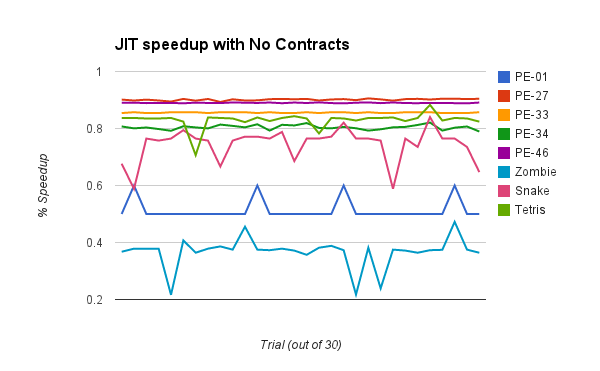
\includegraphics[width=\textwidth]{data/nocontracts-jit-speedup.png}
  \caption{Percent difference in runtimes with and without the JIT}
  \label{speedups}
  \end{center}
\end{figure}
